\documentclass{article}
\usepackage{graphicx}
\usepackage{siunitx}
\graphicspath{ {images/} }
\title{Sign Problem}
\author{Grant Curell}
\begin{document}
\maketitle{}
\section{Problem}
For example, take a look at Figure 5-9, where you’ve started your own grocery store and bought a wire rated at 15 newtons to hang the sign with. The sign weighs only 8.0 newtons, so hanging it should be no problem, right? Obviously, you can tell from my phrasing that you have a problem here. Coolly, you get out your calculator to figure out what force the wire, F1 in the diagram, has to exert on the sign to support it.

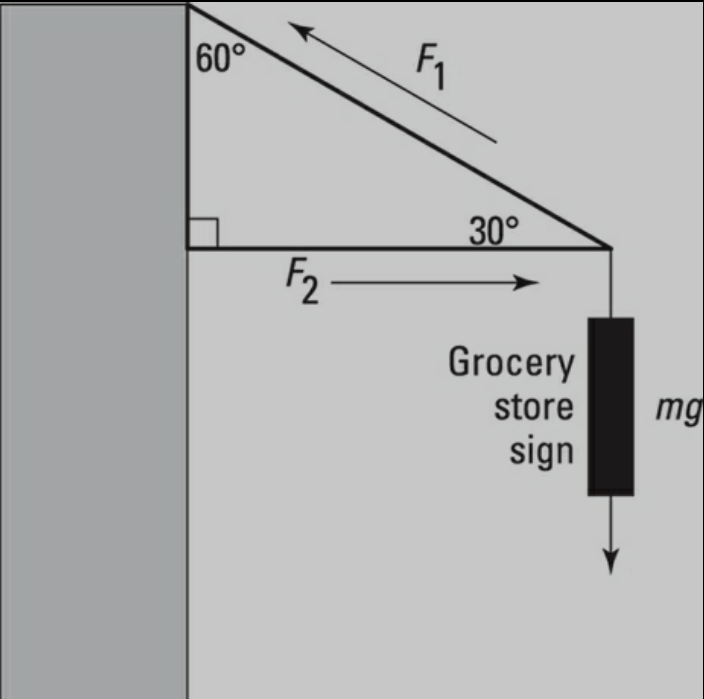
\includegraphics[width=\columnwidth]{image}
\\\\
Holzner, Steven. Physics I For Dummies (For Dummies (Math \& Science)) (p. 97). Wiley. Kindle Edition.
\\\\
\section{Solution}
\[ F_1=15N \]
\[ F_s=8N \]
\[ a=0 \]
\[ F_{sign-y}=15\cos(60) \]
\[ F_{sign-y}=7.5 \]
El letrero require 8N de fuerza para sostenerse. El alambre solo puede apoyar 7.5N de fuerza en la eje y lo que es insuficiente.
\\\\
The sign requires 8N of force to support itself. The wire can only support 7.5N in the y axis, which is insufficient for the 8N required by the wire.
\section{Question}
The book used the following explanation. Mine seems logical, but is it mathematically correct?
\\\\
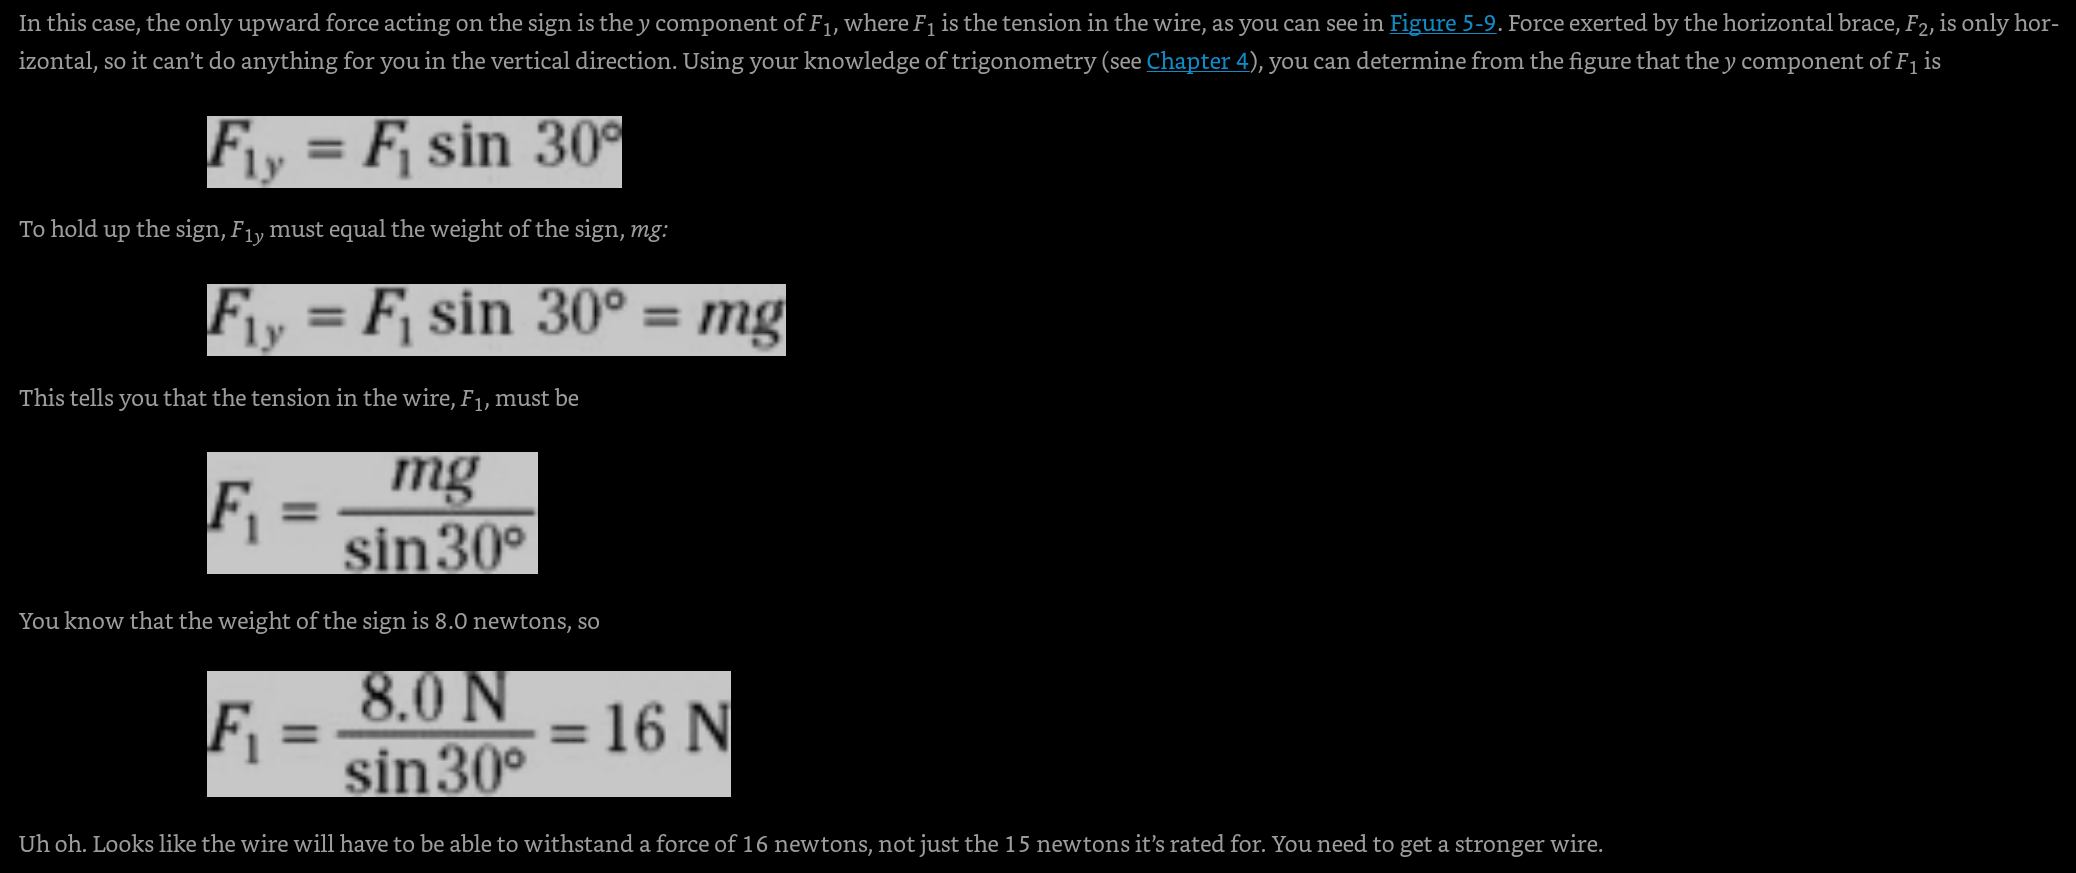
\includegraphics[width=\columnwidth]{image2}
\end{document}
